% \chapter{Background}\label{Background}
% Explain what the reader needs to understand your work.

% Everything needed to understand your design goes here,
% but nothing specific to your implementation.

% Good content here:

% constellation diagrams

% equations

% algorithm explanation

% references to papers

% block diagrams
% \section{Coherent optical communication systems}
% Traditional short-reach optical links in datacenters are typically based on 
% \ac{IMDD}. In \ac{IMDD} systems, information 
% is only encoded in the optical power of the transmitted signal, while the receiver 
% directly measures the incoming optical intensity using a photodiode. \todo{explain how this is done}

% \missingfigure{working princinple of IMDD receivers}

% IMDD links 
% are relatively simple and energy-efficient, making them attractive for short 
% distances and moderate data rates. However, they become increasingly difficult to 
% scale towards higher capacities because chromatic dispersion, limited spectral 
% efficiency and the inability to exploit both amplitude and phase dimensions begin 
% to dominate the system performance.\todo{explain why chromatic dispersion arises, as well as
% what spectral efficiency is and why it is limited for higher capacities}
% \\\\
% Coherent optical communication systems overcome these limitations by detecting 
% both the amplitude and phase of the optical field. This enables the use of 
% advanced modulation formats such as \ac{QPSK}, \ac{16QAM} and higher-order 
% constellations, significantly increasing the amount of information that can be 
% transmitted per symbol. In addition, coherent receivers can digitally compensate 
% for channel impairments such as chromatic dispersion and polarization effects, 
% making them highly attractive for future intra-datacenter interconnects where 
% bandwidth requirements continue to increase. Coherent optical communication is 
% therefore increasingly being considered as a replacement for IMDD in short-reach 
% high-capacity links. [INSERT REF] \todo{insert ref USAGE IMDD VS COHERENT}
% \\\\
% A simplified coherent receiver consists of an incoming optical signal, a local 
% oscillator laser and a \(90^\circ\) optical hybrid followed by balanced 
% photodiodes \todo{optical hybrid? balanced photodiode? explain terms}. The local oscillator mixes with the received optical field, such 
% that both the in-phase and quadrature components of the signal can be recovered. 
% The resulting electrical signal is digitized and further processed in the digital 
% signal processing chain.
% \\\\
% After analog-to-digital conversion, the coherent receiver typically performs 
% several \ac{DSP} operations, including chromatic dispersion compensation, timing 
% recovery, adaptive equalization, carrier frequency recovery and carrier phase 
% recovery. Carrier recovery is usually one of the final stages in the DSP chain, 
% because it assumes that the received symbols have already been equalized and 
% mapped close to their ideal constellation locations. \todo{is this true? confirm}
% \\\\
% The use of free-running lasers at both transmitter and receiver introduces an 
% important challenge. The transmitter laser and local oscillator laser are never 
% perfectly matched in frequency or phase. As a consequence, the received 
% constellation continuously rotates over time, making correct symbol decisions 
% impossible unless this phase rotation is estimated and compensated digitally. 
% This is one of the central challenges addressed in this thesis. Digital coherent 
% systems therefore rely on efficient carrier recovery algorithms. 
% Carrier recovery has traditionally been performed using analog phase-locked 
% loops, but modern coherent systems instead perform this operation digitally, 
% since digital methods are more robust against instabilities and polarization 
% effects. [INSERT REF] \todo {insert ref CARRIER RECOVERY SYSTEMS}


% \section{Phase noise and frequency offset}
% The main phase-related impairments in coherent optical communication systems are 
% carrier frequency offset and phase noise. Both arise because the transmitter and 
% local oscillator lasers are independent devices and therefore do not share an 
% identical optical frequency or phase reference.
% \\\\
% Carrier frequency offset occurs because the optical carrier frequency of the 
% transmitter laser differs slightly from that of the local oscillator laser. In 
% intradyne coherent systems, this mismatch can still amount to several hundreds of 
% megahertz or even a few gigahertz. After coherent detection, this difference 
% appears as a constant phase increment between consecutive received symbols. 
% Consequently, the received constellation rotates steadily over time. 
% Mathematically, this phase rotation can be expressed as

% \begin{equation}
% y[k] = s[k] e^{j(\theta[k] + 2\pi \Delta f T_s k)} + \eta[k]
% \end{equation}

% where \(s[k]\) is the transmitted symbol, \(\theta[k]\) is the phase noise, 
% \(\Delta f\) is the carrier frequency offset, \(T_s\) is the symbol period and 
% \(\eta[k]\) is additive noise. [INSERT REF] \todo{insert ref CURSUS}
% \\\\
% The term \(2\pi \Delta f T_s k\) corresponds to a linear phase ramp. A larger 
% frequency offset or a larger symbol duration leads to faster constellation 
% rotation. This is particularly relevant for block-based carrier recovery systems, 
% because the total accumulated phase change within one block determines whether 
% phase ambiguities and cycle slips can occur.
% \\\\
% Besides frequency offset, coherent optical systems are also affected by phase 
% noise. Phase noise originates from spontaneous emission inside the lasers and is 
% typically modelled as a Wiener process. Unlike frequency offset, which produces a 
% deterministic linear phase drift, phase noise is random and accumulates over 
% time. The phase noise variance increases with the combined linewidth of the 
% transmitter and local oscillator lasers. In practice, the discrete-time phase 
% noise process can be written as

% \begin{equation}
% \theta[k] = \theta[k-1] + \Delta \theta[k]
% \end{equation}

% where \(\Delta \theta[k]\) is a random increment with Gaussian statistics. This 
% means that phase noise behaves as a random walk, causing the received 
% constellation to jitter around its average phase position. [INSERT REF] \todo{insert ref CURSUS}
% \\\\
% For the systems considered in this thesis, the residual carrier frequency offset 
% after coarse frequency recovery is especially important. While a separate 
% frequency recovery stage can compensate most of the carrier frequency offset, a 
% small leftover frequency error remains due to the finite resolution of the 
% estimator. This residual offset causes a nearly linear phase drift across each 
% DSP block.
% \missingfigure{figure illustrating the near-lineair approximation 
% of the total noise process}

% The phase recovery system must therefore not only compensate random 
% phase noise caused by laser linewidth, but also account for this remaining 
% within-block phase slope. This motivates the channel model used throughout this 
% thesis, in which the received symbols are impaired by:

% \begin{itemize}
%     \item additive white Gaussian noise,
%     \item a residual carrier frequency offset,
%     \item Wiener phase noise caused by laser linewidth.
% \end{itemize}

% A coarse fourth-power FFT-based frequency recovery algorithm is often used before 
% phase recovery. For a QPSK signal \(z[k]\), raising the symbols to the fourth 
% power removes the modulation, allowing the dominant residual frequency offset to 
% be estimated from the spectrum:

% \begin{equation}
% z[k]^4 \propto e^{j 8 \pi \Delta f T_s k}
% \end{equation}

% The estimated frequency offset can then be compensated digitally. However, the 
% accuracy of this estimate depends on the FFT size. A finite FFT resolution leads 
% to a remaining frequency estimation error:

% \begin{equation}
% \Delta f_e \leq \frac{F_s}{2N_{\mathrm{FFT}}}
% \end{equation}

% \missingfigure{add figure explaining frequency error due to finite FFT leads to 
% offloading to phase recovery stage}
% This remaining frequency error is then passed on to the phase recovery stage. If 
% the residual offset is too large, the phase recovery block may no longer be able 
% to track the constellation rotation correctly, causing cycle slips.


% \section{Carrier recovery in DSP chains}
% Carrier recovery is the DSP stage responsible for compensating the phase 
% rotations introduced by residual \ac{CFO} and phase noise. Since 
% these impairments have different characteristics, coherent receivers usually 
% perform carrier recovery in two stages.
% \\\\
% The first stage is frequency recovery. Its purpose is to estimate and remove the 
% dominant \ac{CFO} between transmitter and the \ac{LO}. This 
% can be implemented either before or after equalization. Frequency-domain methods 
% typically offer a large acquisition range but only coarse accuracy, while 
% time-domain methods offer finer estimation but require a cleaner signal. As a 
% result, practical coherent receivers often use a coarse frequency-domain 
% estimator followed by a fine time-domain estimator. [INSERT REF] \todo{insert ref
% FREQUENCY RECOVERY METHODS}
% \\\\
% After coarse frequency recovery, the signal still contains residual \ac{CFO} and phase noise. 
% These impairments are then handled by the second stage, 
% namely phase recovery. Unlike frequency recovery, phase recovery operates on a 
% symbol-by-symbol or block-by-block basis and attempts to track the residual 
% rotation of the constellation. \todo{explain how frequency recovery doesn't work on a 
% symbol or block basis}
% \\\\
% A major challenge is that modern coherent DSP systems process many symbols in 
% parallel in order to reduce clock speed requirements. As a result, carrier phase 
% is often estimated only once per processing block instead of once per symbol. 
% Although this significantly reduces computational complexity, it also increases 
% the sensitivity to phase drift within the block. If the total phase change over a 
% block becomes too large, the phase recovery algorithm may interpret the 
% constellation incorrectly and introduce a cycle slip. For square QAM 
% constellations, this typically corresponds to a phase ambiguity of \(\pi/2\). 
% Once a cycle slip occurs, the entire constellation rotates by \(\pi/2\), leading 
% to a large number of bit errors.
% \\\\
% The maximum recoverable phase change over a processing block is therefore limited 
% by the unwrapping threshold. If a block contains \(B\) symbols and the residual 
% frequency offset is \(\Delta f_e\), the total phase drift across the block can be 
% approximated by

% \begin{equation}
% \Delta \phi_{\mathrm{block}} \approx 2 \pi \Delta f_e B T_s
% \end{equation}

% To avoid cycle slips, this accumulated phase should remain smaller than the phase 
% ambiguity threshold of the phase unwrapping system. In conventional blind phase 
% search systems, this often translates into a requirement that the total phase 
% drift over a block must remain below approximately \(\pi/4\). [INSERT REF] \todo{insert ref BPS TRACKING RANGE}

% \section{Blind Phase Search}
% \Ac{BPS} is one of the most widely used carrier phase recovery 
% algorithms for coherent QAM systems. The method is feedforward and does not rely 
% on pilot symbols, making it attractive for high-throughput coherent receivers. \todo{find ref for why bps is attractive?}
% \\\\
% The principle of BPS is relatively straightforward. A block of received symbols is 
% rotated over a number of candidate test angles. For each candidate angle, the 
% rotated symbols are sliced to the nearest ideal constellation points and an error 
% metric is computed. The candidate angle that minimizes the total error is then 
% selected as the estimated carrier phase.

% \missingfigure{block diagram of working bps principle + testangles on constellationdiagram}

% For a received block \(z[k]\), the BPS metric for a test phase \(\phi\) can be 
% written as

% \begin{equation}
% e(\phi) = \sum_{k=0}^{B-1} \left| D\left(z[k] e^{-j\phi}\right) - z[k] e^{-j\phi} \right|^2
% \end{equation}

% where \(D(\cdot)\) denotes the decision operation that maps a rotated symbol to 
% its nearest constellation point. The phase estimate is then given by the test 
% angle that minimizes \(e(\phi)\).
% \\\\
% For square QAM constellations, only the phase interval 
% \([-\pi/4, \pi/4]\) needs to be searched because of the \(\pi/2\) rotational 
% symmetry of the constellation\todo{elabore further}. However, a large number of test phases is usually 
% required to obtain sufficient estimation accuracy. This makes BPS computationally 
% expensive, especially for high-speed FPGA implementations.
% \\\\
% Another important limitation of BPS is that it only estimates one average phase 
% per block. As a result, it assumes that all symbols in the block experience 
% approximately the same phase rotation. This assumption becomes less valid when 
% the residual frequency offset is large, since the phase can drift significantly 
% from the first to the last symbol in the block. In such cases, a single blockwise 
% phase estimate is insufficient and can lead to incorrect unwrapping decisions and 
% cycle slips. This thesis therefore extends the traditional BPS approach by also 
% estimating the phase spread across the block, which will be explained in chapter \ref{Proposed phase recovery architecture}.
% [INSERT REF] \todo{insert REF LIMITATIONS OF BPS}

% \section{16QAM representations in DSP hardware}
% In FPGA-based DSP systems, complex symbols are represented using fixed-point 
% formats rather than floating-point arithmetic. Fixed-point arithmetic offers much 
% lower hardware complexity, reduced power consumption and more predictable timing, 
% which is essential for high-speed coherent receivers.

% For normalized \ac{16QAM}, the ideal constellation consists of the symbol levels

% \begin{equation}
% \{\pm 1, \pm 3\}
% \end{equation}

% on both the in-phase and quadrature axes. To obtain unit average power, the 
% constellation is scaled by a normalization factor. In practical fixed-point DSP 
% implementations, the resulting symbol amplitudes are then mapped to a signed 
% integer representation such as Q1.15.
% \\\\
% The fixed-point representation directly affects numerical precision, quantization 
% noise and overflow behaviour. A larger word length improves estimation accuracy 
% but also increases hardware complexity. The chosen representation therefore 
% depends on the required balance between accuracy and implementation cost.
% \\\\
% In this thesis, received symbols are represented in Q1.15 format, while phase 
% values are represented in a higher precision Q4.28 format. This distinction is 
% necessary because phase accumulation and trigonometric operations require a larger 
% dynamic range and finer precision than the raw constellation symbols. Additional 
% formats are used internally for trigonometric values, \ac{CORDIC} phase inputs and 
% intermediate multiplication results

% \section{CORDIC}
% The \ac{CORDIC} algorithm is a hardware-
% efficient method to calculate trigonometric functions and perform vector 
% rotations. Instead of relying on expensive multipliers, the algorithm uses only 
% additions, subtractions, bit shifts and lookup tables. This makes it particularly 
% well suited for FPGA implementations.
% \\\\
% In vector rotation mode, the CORDIC algorithm iteratively rotates an input vector 
% over a desired angle by decomposing the total rotation into a sequence of smaller 
% elementary rotations. Each elementary rotation is selected such that it can be 
% implemented using only a shift operation:

% \begin{equation}
% x_{i+1} = x_i - d_i y_i 2^{-i}
% \end{equation}

% \begin{equation}
% y_{i+1} = y_i + d_i x_i 2^{-i}
% \end{equation}

% \begin{equation}
% z_{i+1} = z_i - d_i \arctan(2^{-i})
% \end{equation}

% where \(d_i \in \{-1, +1\}\) determines the direction of rotation at iteration 
% \(i\). After a sufficient number of iterations, the vector is rotated by the 
% desired angle with good precision.
% \\\\
% In the architecture proposed in this thesis, the CORDIC is used to rotate the 
% received \ac{16QAM} symbols by the estimated carrier phase. Since the carrier 
% phase is estimated separately for multiple sections of the block, the CORDIC is 
% used repeatedly to apply the corresponding phase correction to each symbol group.
% \\\\
% Unlike the other algorithmic blocks proposed in this thesis, the CORDIC is not 
% developed from scratch but is based on an existing FPGA \ac{IP} core. Its use 
% therefore mainly requires selecting the appropriate fixed-point formats, pipeline 
% depth and interface signals rather than deriving a new algorithmic implementation.

\chapter{Background}\label{Background}
This chapter summarises the background required to contextualise the proposed coherent
receiver carrier-recovery architecture. It focuses on (i) short-reach IM/DD links versus
coherent detection, (ii) phase-related impairments (carrier frequency offset and laser
phase noise), and (iii) representative DSP-based carrier recovery methods used in coherent
receivers %\cite{Savory2010JSTQE,Kuschnerov2009JLT}.

\section{Coherent optical communication systems}
Traditional short-reach optical interconnects in data centres have often favoured
intensity-modulation/direct-detection (IM/DD) transceivers because they enable simple and
power-efficient receiver front-ends. In IM/DD systems,
information is conveyed by modulating the received optical intensity (or optical power).
At the receiver, a photodiode converts incident optical power into an electrical
photocurrent (square-law photodetection), so the receiver directly observes intensity but
does not directly access the optical carrier phase \cite{Wartak2013OpticalReceivers,KahnHo2004JSTQE}.

IM/DD links are attractive for short distances and moderate data rates; however, as symbol
rates increase, fibre chromatic dispersion becomes increasingly detrimental because group
delay varies with optical wavelength, causing waveform distortion and frequency-selective
fading for intensity-modulated signals. In addition, the achievable spectral efficiency
(information rate per unit bandwidth, in b/s/Hz) is fundamentally constrained when only
intensity is detected, because direct detection effectively exploits fewer degrees of
freedom than coherent detection \cite{KahnHo2004JSTQE}.
 
Coherent optical communication systems overcome these limitations by detecting both the
amplitude and phase of the optical field and enabling advanced modulation formats such as
QPSK and square M-QAM. Coherent detection also supports digital compensation of linear
channel impairments (e.g., chromatic dispersion and polarization effects) in the electrical
domain \cite{KahnHo2004JSTQE,Savory2010JSTQE,Kuschnerov2009JLT}. Recent work on data-centre
optics evaluates when coherent detection becomes favourable relative to IM/DD as per-lane
rates scale, highlighting the trade-off between coherent DSP power/complexity and improved
spectral efficiency and impairment tolerance \cite{Zhou2020JLT}.

A typical intradyne coherent receiver combines the received optical field with a local
oscillator (LO) laser in a 90$^\circ$ optical hybrid. The hybrid generates orthogonal
interference terms that are detected by balanced photodiode pairs, yielding electrical
in-phase (I) and quadrature (Q) components. Balanced detection improves sensitivity to the
desired beating term and suppresses common-mode intensity noise \cite{Savory2010JSTQE,Kikuchi2016JLT}.

After analog-to-digital conversion, the coherent receiver typically performs several DSP
operations, including chromatic dispersion compensation, timing recovery, adaptive
equalization, carrier frequency recovery and carrier phase recovery \cite{Savory2010JSTQE,Kuschnerov2009JLT}.
In many DSP chains, dispersion compensation and polarization demultiplexing/equalization
are performed prior to carrier phase estimation because commonly used blind equalizers can
converge without an explicit carrier-phase reference; in practice, frequency-offset
estimation may be placed either before or after equalization depending on acquisition range
and implementation constraints \cite{Savory2010JSTQE,Kuschnerov2009JLT}.

Historically, optical coherent receivers often relied on analogue phase-locked loops (PLLs)
for carrier synchronisation. In modern DSP-based coherent receivers, carrier recovery is
commonly implemented digitally using feed-forward and/or decision-directed algorithms,
which avoids tight analogue loop dynamics and integrates naturally with polarization-diverse
digital processing \cite{Savory2010JSTQE,IpKahn2007JLT,Pfau2009JLT}.

\section{Phase noise and frequency offset}\label{phase noise and frequency offset}
The main phase-related impairments in coherent optical communication systems are carrier
frequency offset (CFO) and phase noise. Both arise because the transmitter and local
oscillator lasers are independent devices and therefore do not share an identical optical
frequency or phase reference \cite{Kikuchi2016JLT}.

Carrier frequency offset occurs because the instantaneous optical frequency of the
transmitter laser differs from that of the LO laser. After coherent detection and
digitisation, CFO appears as an effective baseband frequency offset and produces a
deterministic phase ramp across samples \cite{Kikuchi2016JLT}. Mathematically,
this phase rotation can be expressed as
\begin{equation}
y[k] = s[k] e^{j(\theta[k] + 2\pi \Delta f T_s k)} + \eta[k]
\end{equation}
where $s[k]$ is the transmitted symbol, $\theta[k]$ is the phase noise, $\Delta f$ is the
carrier frequency offset, $T_s$ is the symbol period and $\eta[k]$ is additive noise
\cite{Kikuchi2016JLT,RoudasCoherentSystems}.

The term $2\pi \Delta f T_s k$ corresponds to a linear phase ramp. A larger frequency offset
or a larger symbol duration leads to faster constellation rotation. This is particularly
relevant for block-based carrier recovery systems, because the total accumulated phase
change within one block influences the probability of phase ambiguities and cycle slips
\cite{Pfau2009JLT}.

Besides frequency offset, coherent optical systems are also affected by phase noise. Laser
phase noise is commonly modelled as a discrete-time Wiener process (random walk) \cite{RoudasCoherentSystems}:
\begin{equation}
\theta[k] = \theta[k-1] + \Delta \theta[k]
\end{equation}
where $\Delta\theta[k]$ is a zero-mean Gaussian increment whose variance is proportional to
the combined (beat) linewidth and the sampling interval \cite{RoudasCoherentSystems,Pfau2009JLT}.

For the systems considered in this thesis, the residual CFO after coarse frequency recovery
is especially important. While a separate frequency recovery stage can compensate most of
the CFO, a small leftover frequency error remains due to the finite resolution of practical
estimators \cite{Leven2007LPT,Selmi2009ECOC}. This residual offset causes a nearly linear
phase drift across each DSP block.

\begin{figure}[H]
\centering
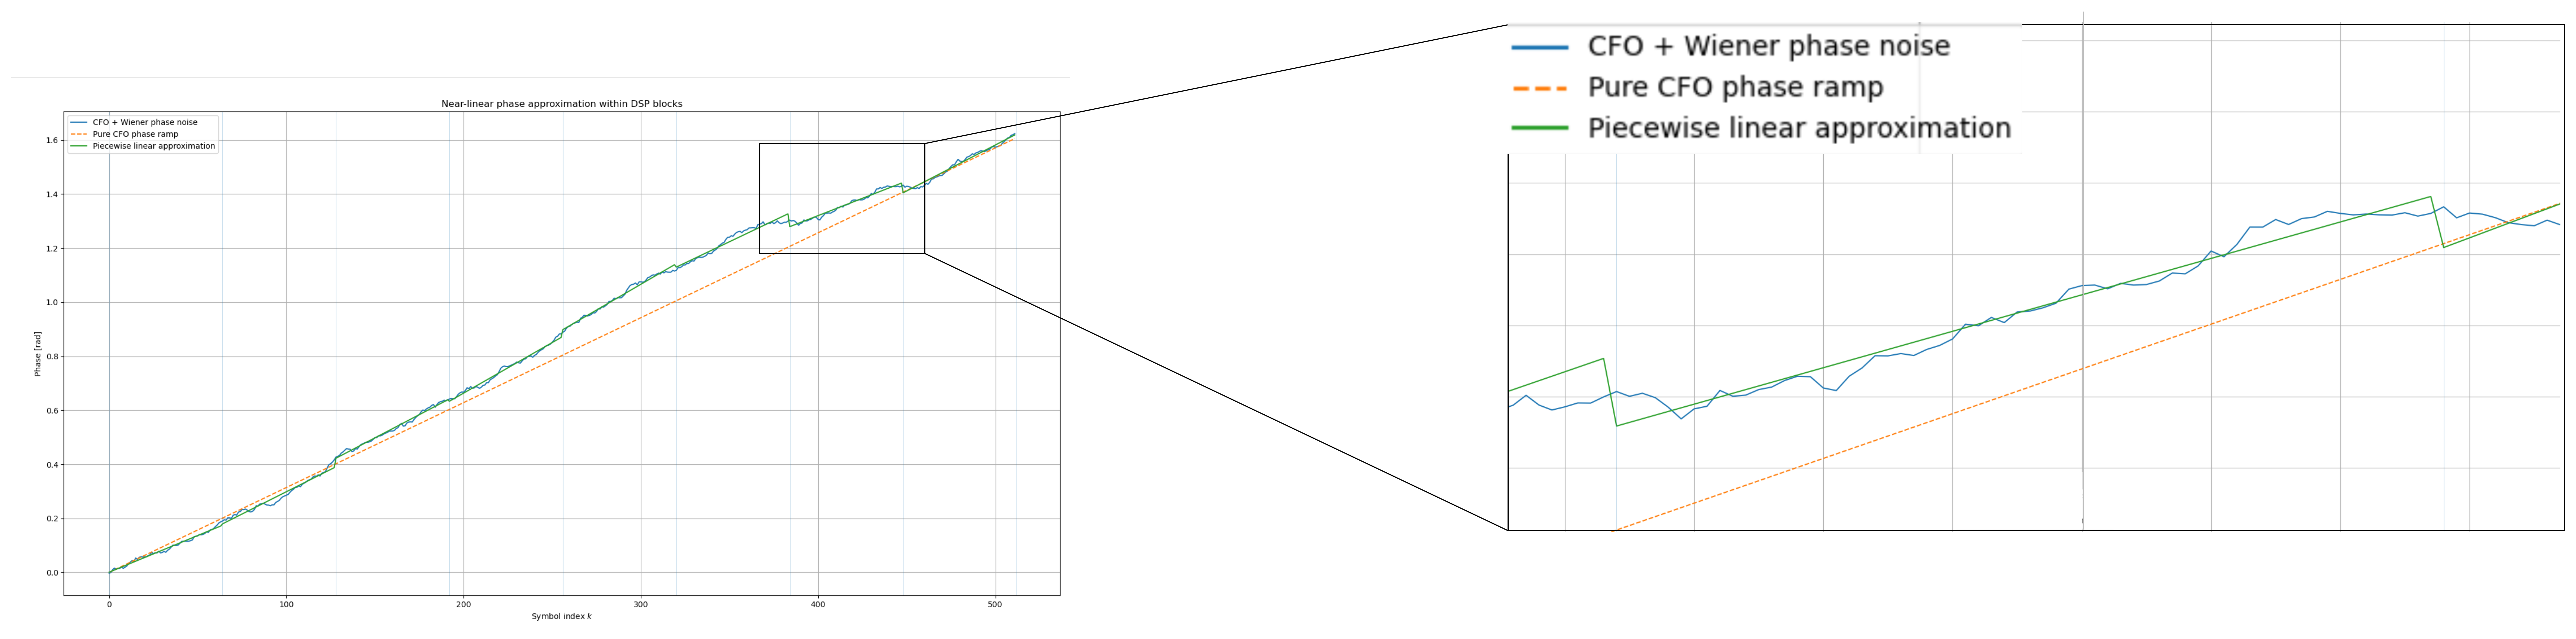
\includegraphics[width=1\linewidth]{figures/linear_approx.png}
\caption{Near-lineair approximation
of the total noise process ($ \Delta f = 16 \text{MHz} $, dnu = $ 0.1 \text{MHz} $, baud = $ 32 \text{GBaud} $)}
\label{fig:linear_approx}
\end{figure}
\todo{clean up figure, legend}


The phase recovery system must therefore not only compensate random phase noise caused by
laser linewidth, but also account for remaining within-block phase slope. This motivates
the channel model used throughout this thesis, in which the received symbols are impaired by:
\begin{itemize}
    \item additive white Gaussian noise,
    \item a residual carrier frequency offset,
    \item Wiener phase noise caused by laser linewidth.
\end{itemize}

A coarse FFT-based frequency recovery algorithm is often used before phase recovery.
FFT-based CFO estimation provides wide acquisition range at modest complexity
\cite{Leven2007LPT,Selmi2009ECOC}. For M-PSK constellations, an M-th power nonlinearity can
suppress the data modulation and expose a strong carrier-related spectral line that enables
peak-based CFO estimation; related techniques are also adapted for square QAM via
partitioning, pilots, or data-aided processing \cite{Rasmussen2011SPIE}.

The estimated frequency offset can then be compensated digitally. However, the accuracy of
this estimate depends on the FFT size. A finite FFT resolution leads to a remaining
frequency estimation error. Since the FFT bin spacing equals $F_s/N_{\mathrm{FFT}}$, a
simple bin-centred peak estimate implies an error on the order of half a frequency bin:
\begin{equation}\label{eq: frequency recovery bin size error}
\Delta f_e \leq \frac{F_s}{2N_{\mathrm{FFT}}}
\end{equation}
\cite{AnalogDevicesDFT,AgilentNoiseGuide}.

\begin{figure}[H]
\centering
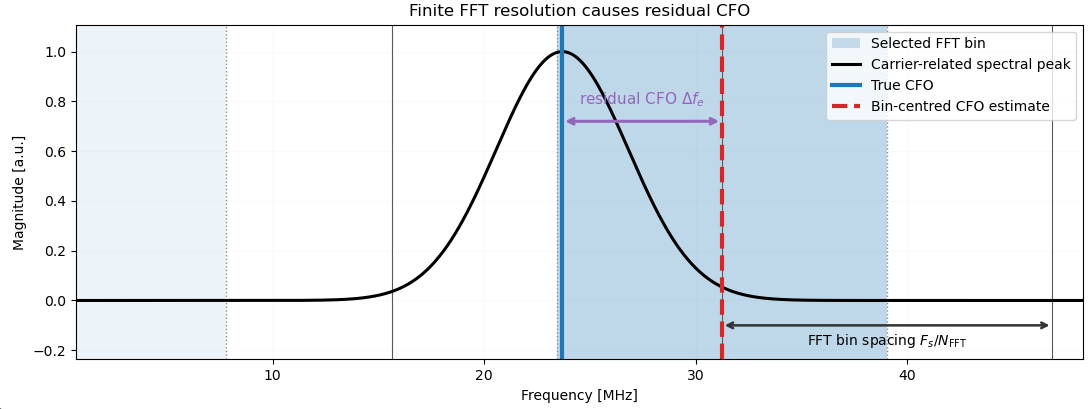
\includegraphics[width=1\linewidth]{figures/FFT-resolution.png}
\caption{FFT-binsize leading to residual phase offset ($ F_s = 32 \text{GHz} $, $ N_{FFT} = 2048 $)}
\label{fig:FFT-resolution}
\end{figure}

This remaining frequency error is then passed on to the phase recovery stage. If the
residual offset is too large, the phase recovery block may no longer be able to track the
constellation rotation correctly, which increases the probability of cycle slips
\cite{Pfau2009JLT,Kuschnerov2009JLT}.

\section{Carrier recovery in DSP chains}\label{carrier recovery in DSP chains}
Carrier recovery is the DSP stage responsible for compensating the phase rotations
introduced by residual CFO and phase noise. Since these impairments have different
characteristics, coherent receivers commonly separate carrier recovery into (i) frequency
offset estimation/compensation and (ii) carrier phase estimation \cite{Savory2010JSTQE,Kuschnerov2009JLT}.

Frequency recovery estimates a single CFO parameter over an observation interval and
therefore benefits from aggregating many samples to improve estimator variance;
it is not typically meaningful to produce an independent CFO estimate per symbol. By
contrast, carrier phase recovery must track a time-varying phase process (Wiener phase
noise plus residual CFO), motivating symbol-rate or block-rate phase estimation\cite{Leven2007LPT,Pfau2009JLT}.

A major challenge is that modern coherent DSP systems process many symbols in parallel in
order to reduce clock speed requirements. As a result, carrier phase is often estimated
only once per processing block instead of once per symbol \cite{Kuschnerov2009JLT}. Although
this significantly reduces computational complexity, it also increases sensitivity to phase
drift within the block. If the total phase change over a block becomes too large, the phase
recovery algorithm may unwrap to an incorrect $\pi/2$-shifted hypothesis (cycle slip) for
square QAM constellations \cite{Pfau2009JLT}.

If a block contains $B$ symbols and the residual frequency offset is $\Delta f_e$, the total
phase drift across the block can be approximated by
\begin{equation}
\Delta \phi_{\mathrm{block}} \approx 2 \pi \Delta f_e B T_s
\end{equation}
To reduce the probability of cycle slips, a practical design rule is to keep the intra-block
phase drift well below the midpoint between neighbouring $\pi/2$-ambiguous hypotheses, often
expressed as $|\Delta \phi_{\mathrm{block}}| \lesssim \pi/4$ \cite{Pfau2009JLT}.

\section{Blind Phase Search}\label{background: blind phase search}
Blind Phase Search (BPS) is a widely used feed-forward carrier phase estimation method for
coherent square M-QAM. Its advantages include pilot-free operation, modulation-format
compatibility, and strong tolerance to laser phase noise when sufficient test phases and
averaging are used \cite{Pfau2009JLT,Yang2018OE}.

The principle of BPS is straightforward. A block of received symbols is rotated over a set
of candidate test angles. For each candidate angle, the rotated symbols are sliced to the
nearest ideal constellation points and an error metric is computed. The candidate angle
that minimises the total error is selected as the estimated carrier phase \cite{Pfau2009JLT}.

\begin{figure}[H]
\centering
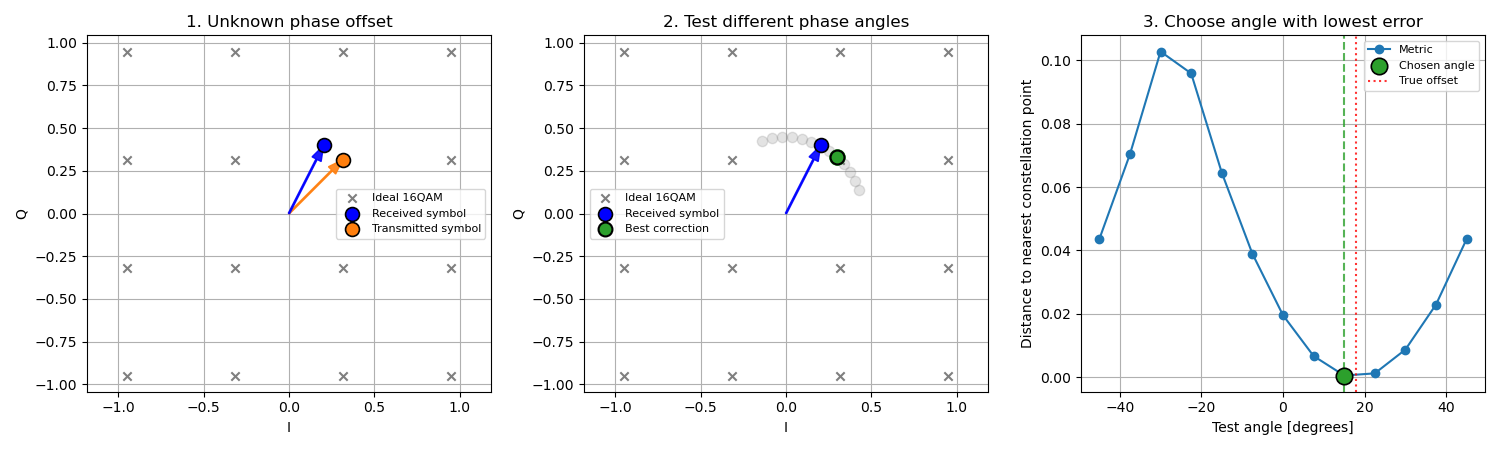
\includegraphics[width=1\linewidth]{figures/BPS_working_principle.png}
\caption{Working BPS principle}
\label{fig:BPS-principle}
\end{figure}

For a received block $z[k]$, the BPS metric for a test phase $\phi$ can be written as
\begin{equation}
e(\phi) = \sum_{k=0}^{B-1} \left| D\left(z[k] e^{-j\phi}\right) - z[k] e^{-j\phi} \right|^2
\end{equation}
where $D(\cdot)$ denotes the decision operation that maps a rotated symbol to its nearest
constellation point. The phase estimate is then given by the test angle that minimises
$e(\phi)$.

For square QAM constellations, the objective function in BPS is periodic with period $\pi/2$
due to constellation rotational symmetry. Therefore, it suffices to search any interval of
length $\pi/2$; a common centred choice is $[-\pi/4,\pi/4]$ \cite{Pfau2009JLT}. However, a
large number of test phases is usually required to obtain sufficient estimation accuracy,
making BPS computationally expensive in high-throughput FPGA implementations
\cite{Pfau2009JLT,Yang2018OE}.

Another limitation of blockwise BPS is that it estimates one average phase per block. When
residual CFO induces significant intra-block phase drift, a single blockwise estimate can be
insufficient and may increase cycle-slip probability \cite{Pfau2009JLT}. This thesis therefore
extends the traditional blockwise BPS approach by also estimating the phase spread across the
block, as explained in Chapter~\ref{Proposed phase recovery architecture}.

\section{CORDIC}
The Coordinate Rotation Digital Computer (CORDIC) algorithm implements vector rotations and
elementary functions using iterative shift-add operations. Its attractiveness in FPGA/ASIC
implementations stems from replacing general multipliers with pipelinable add/subtract and
bit-shift datapaths \cite{Volder1959TEC,Meher2009TCASI}.

In the rotation mode of CORDIC, a vector is iteratively rotated by a sequence of predefined
micro-rotations. The iterative equations can be written as \cite{Volder1959TEC,Meher2009TCASI}:
\begin{equation}
x_{i+1} = x_i - d_i y_i 2^{-i}
\end{equation}
\begin{equation}
y_{i+1} = y_i + d_i x_i 2^{-i}
\end{equation}
\begin{equation}
z_{i+1} = z_i - d_i \arctan(2^{-i})
\end{equation}
where $d_i \in \{-1, +1\}$ determines the direction of rotation at iteration $i$.
After a sufficient number of iterations, the vector is rotated by the desired angle with
good precision \cite{Meher2009TCASI}.

In this thesis, CORDIC is used to rotate received symbols by the estimated carrier phase.
The implementation leverages an FPGA IP core; design effort therefore focuses on selecting
fixed-point formats, pipeline depth/latency, and interface timing to meet throughput and
numerical-accuracy requirements \cite{AMD2021PG105}.
  